\section{Auswertung}
\label{sec:Auswertung}

%\begin{figure}
%  \centering
%  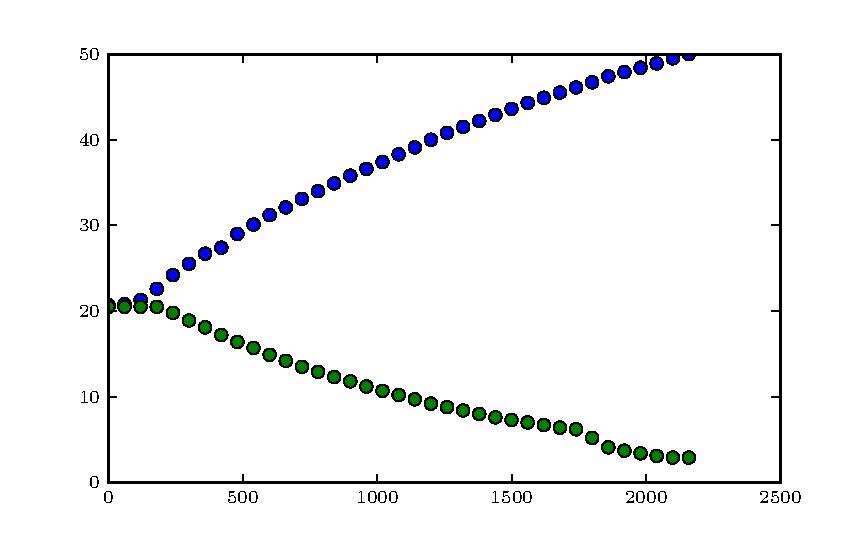
\includegraphics{plot.pdf}
%  \caption{Plot.}
%  \label{fig:plot}
%\end{figure}




%%%%%%%%%%%%%%%%%%%%%%%%%%%%%%%%%%%%%%
%Strömungsprofil
%%%%%%%Pumpleistung 70%
\begin{figure}
  \centering
  \includegraphics{Bilder/f70.pdf}
  \caption{Plot.}
  \label{fig:f70}
\end{figure}
\begin{figure}
  \centering
  \includegraphics{Bilder/I70.pdf}
  \caption{Plot.}
  \label{fig:I70}
\end{figure}

\begin{table}
\centering
\caption{Pumpleistung 70\%}
\label{tab:pl70}
\begin{tabular}{ccc}
  \toprule
Eindringtiefe/$\si{\milli\meter}$ & $I_\mathrm{Streu}$/$\si{\square\volt\per\second}$ & $\Delta \nu$/$\si{\Hz}$ \\
\midrule
19.5 & 90.0 & 439.0 \\
20.25 & 114.0 & 490.0 \\
21.0 & 126.0 & 562.0 \\
21.75 & 140.0 & 623.0 \\
22.5 & 156.0 & 647.0 \\
23.25 & 160.0 & 623.0 \\
24.0 & 176.0 & 574.0 \\
24.75 & 187.0 & 500.0 \\
25.5 & 183.0 & 439.0 \\
26.25 & 206.0 & 421.0 \\
27.0 & 250.0 & 500.0 \\
27.75 & 495.0 & 500.0 \\
28.5 & 438.0 & 500.0 \\
29.25 & 348.0 & 500.0 \\
\bottomrule
\end{tabular}
\end{table}




%%%%%%%Pumpleistung 45%
\begin{figure}
  \centering
  \includegraphics{Bilder/f45-2.pdf}
  \caption{Plot.}
  \label{fig:f45}
\end{figure}
\begin{figure}
  \centering
  \includegraphics{Bilder/I45-2.pdf}
  \caption{Plot.}
  \label{fig:I45}
\end{figure}
\begin{table}
  \centering
  \caption{Pumpleistung 45\%}
  \label{tab:pl45}
\begin{tabular}{ccc}
  \toprule
Eindringtiefe/$\si{\milli\meter}$ & $I_\mathrm{Streu}$/$\si{\square\volt\per\second}$ & $\Delta \nu$/$\si{\Hz}$ \\
\midrule
19.5 & 90.0 & 220.0 \\
20.25 & 120.0 & 232.0 \\
21.0 & 155.0 & 269.0 \\
21.75 & 170.0 & 305.0 \\
22.5 & 180.0 & 317.0 \\
23.25 & 208.0 & 305.0 \\
24.0 & 230.0 & 281.0 \\
24.75 & 203.0 & 269.0 \\
25.5 & 196.0 & 232.0 \\
26.25 & 191.0 & 226.0 \\
27.0 & 232.0 & 244.0 \\
27.75 & 444.0 & 256.0 \\
28.5 & 360.0 & 244.0 \\
29.25 & 300.0 & 256.0 \\
\bottomrule
\end{tabular}
\end{table}
